\chapter{%
デジタルツインシステム}

デジタルツインシステムには物理モデルとそれを模倣したデジタルモデルが必要である.
第2.1章では物理モデルの詳細について,第2.2章ではデジタルモデルの詳細について説明し,
第2.3章ではROSを用いて開発したデジタルツインシステムについて全体像からデジタルツインの対象まで順に追って説明する.


\section{物理モデル}
本節では,デジタルツインシステムにおける物理モデルであるロボットアームと切り紙グリッパーについて述べる.
	
\subsection{ロボットアーム}
まず,物理モデルのロボットアームについて述べる.ロボットアームはUFACTORY社製の6自由度ロボットアームであるLite6を使用する.図2.1にLite6の外観を,表2.1にLite6のハードウェア情報を示す.


\begin{figure}[htbt]
	\centering
	 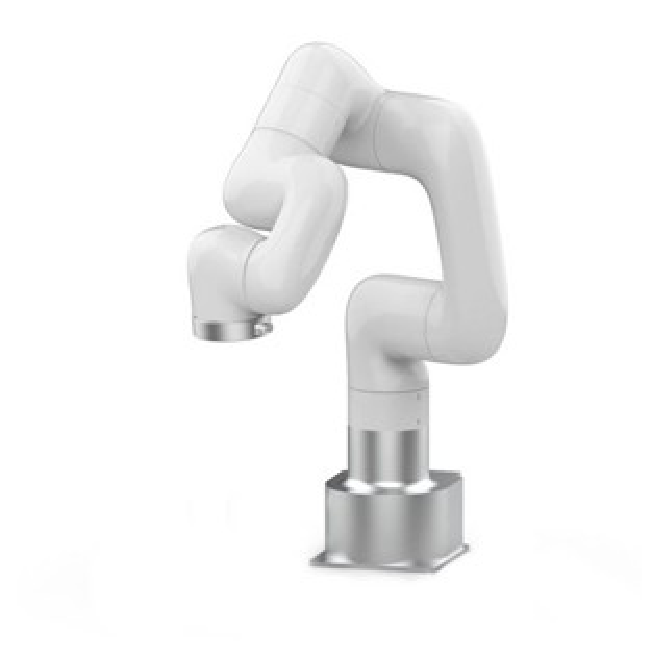
\includegraphics[height=60mm]{lite6.eps}
	 \caption{UFACTORY Lite6}
	 \label{fig:f2}
\end{figure}

\begin{table}[htb]
	\centering
	\caption{Lite6のハードウェア情報}
	\begin{tabular}{lcrc} \hline
	Name          &Value     &Joint Name&Limit Value     \\ \hline \hline
	DOF           & 6        & Joint1   & $\pm360^\circ$ \\
	Weight        & 9kg      & Joint2   & $\pm150^\circ$ \\
	Max Rearch    & 440mm    & Joint3   & ~$-3.5^\circ$--$300^\circ$ \\
	Max Speed     & 500mm/s  & Joint4   & $\pm360^\circ$ \\
	Payload       & 1kg      & Joint5   & $\pm124^\circ$ \\
	Repeatability & 0.2mm    & Joint6   & $\pm360^\circ$ \\ \hline
	\end{tabular}
\end{table}

\subsection{切り紙グリッパー}
次に,物理モデルの切り紙グリッパーについて述べる.前述したように切り紙グリッパーはLiang Duらによって本研究室で開発された.
彼らは厚紙から切り抜いた平面形状の3本の指を持つ紙グリッパーをDYNAMIXEL社製モータXM430-W210とボールねじを組み込んだ装置の先端に取り付け,
モータの回転運動をボールねじで直動運動に変換して伸縮させることで紙グリッパーの開閉を実現した.装置の外装はPLAを3Dプリントして制作された.\\
 本研究では切り紙グリッパーの開閉時の指先の位置を測定するため,素材を強度が低く変形しやすい厚紙から$0.3mm$のPETシートに変更した.
また,切り紙グリッパーの装置への取り付けは,従来はボルトで紙を挟み込むことによる圧着であったが,本研究では圧着していた部分にあらかじめ穴を開けボルトをその穴に通して固定する方法に変更した.
これにより,圧着場所によって切り紙グリッパーの設置位置が変化する問題を解決することができた.
このグリッパーは本研究のために設計,制作された専用のコネクタを介してボルトで接続する.

\begin{figure}[htbt]
	\centering
	 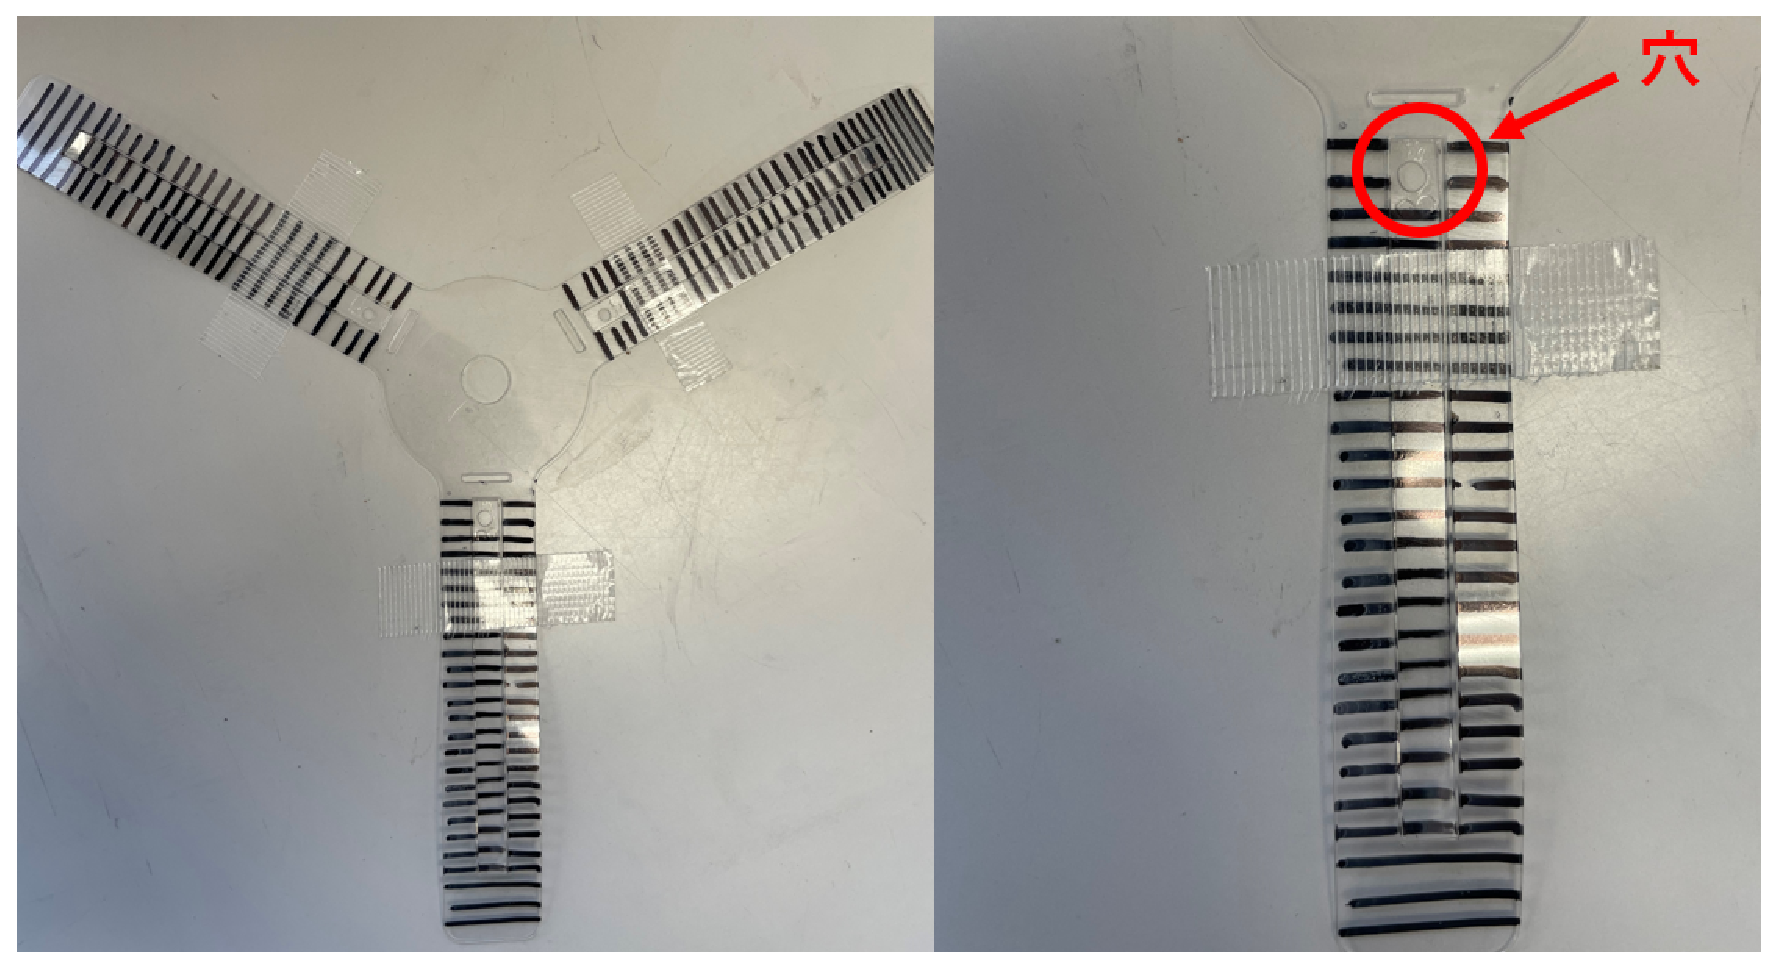
\includegraphics[height=60mm]{pet_gripper.eps}
	 \caption{PETシートから切り抜いた切り紙グリッパー}
	 \label{fig:f2}
\end{figure}
\begin{figure}[htbt]
	\centering
	 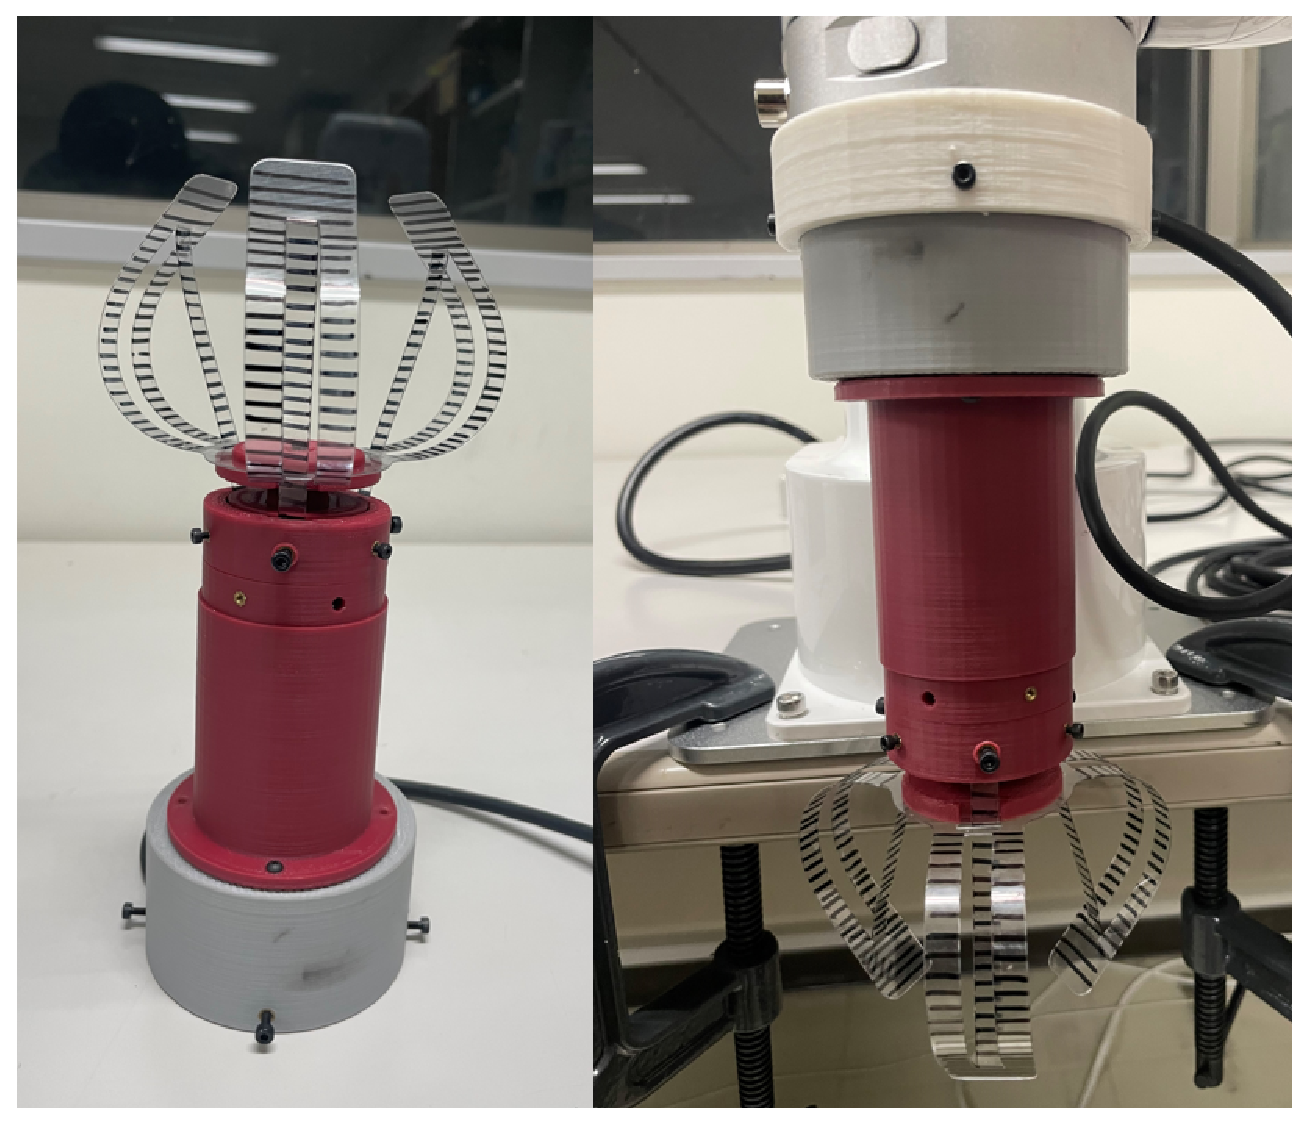
\includegraphics[height=60mm]{kirigami_gripper.eps}
	 \caption{切り紙グリッパーの装置とLite6への接続}
	 \label{fig:f2}
\end{figure}


\section{デジタルモデル}
本節では,切り紙グリッパーを持つロボットアームのデジタルツインシステムにおけるデジタルモデルについて述べる.
物理的なロボットであるUFACTORY Lite6と切り紙グリッパーのデジタルツインモデルをGazeboシミュレータ上に表示するには3DモデルとURDFの作製が必要である.
Lite6の3DモデルとURDFはUFACTORYから公式に提供されているものを使用できたが,切り紙グリッパーはその3DモデルをCADで作製しその構造をURDFで記述する必要があった.
切り紙グリッパーはPET素材のグリッパーが装置の伸縮によって大きく変形するが,その様子をCADとURDFで作製しGazebo上に表示させることは非常に困難である.
そこで,切り紙グリッパーを3本の剛体の指とそれに対応した関節軸を持つグリッパーと見なしてモデリングを行った.\\
 図2.4にROSの3D可視化ツールであるRvizで表示した切り紙グリッパーのモデル(a)と3DモデルとURDFによって作られた切り紙グリッパーを手先に持つLite6をGazebo上に表示した様子(b)を示す.
図から,白色の3本の指が赤色の装置から伸び,指の関節部分に座標軸があることがわかる.

\begin{figure}[htbt]
	\centering
	 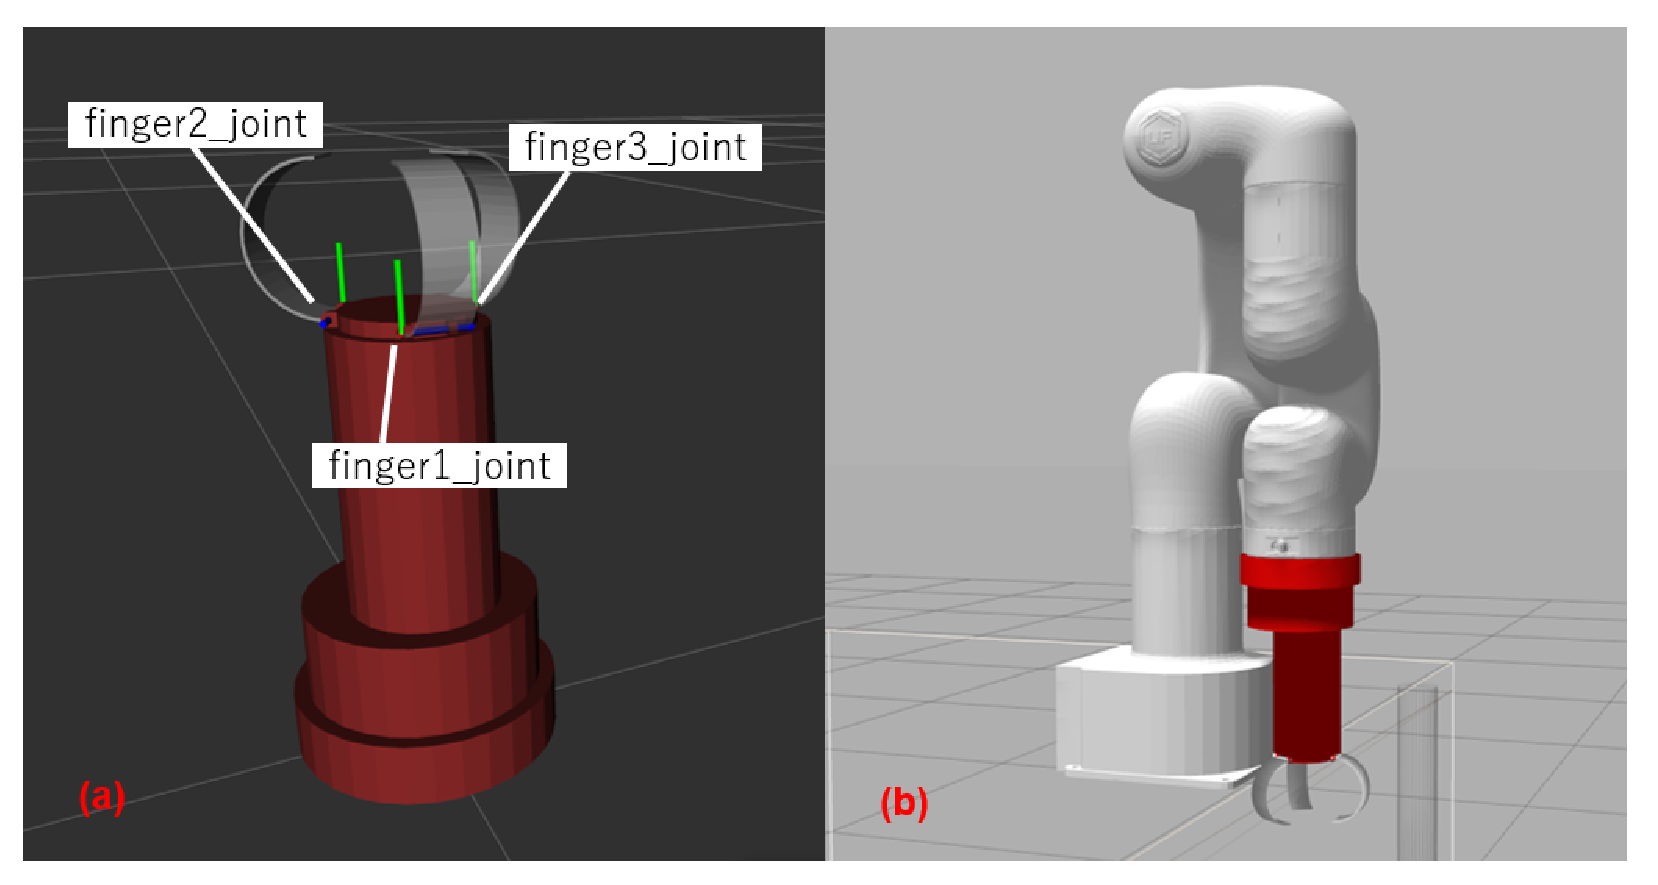
\includegraphics[height=60mm]{kirigami_gripper_rviz_and_lite6_with_kirigami_gripper_gazebo.eps}
	 \caption{Rvizで表示した切り紙グリッパーのモデル(a)とGazeboで表示した切り紙グリッパーを持つLite6のデジタルモデル(b)}
	 \label{fig:f2}
\end{figure}

指の形状は実際の切り紙グリッパーが完全に開いた時と閉じた時の取り付け面から指先までのそれぞれの垂直距離を測り,その差の真ん中の値を直径とした半円弧でモデリングした.\\
 そして,切り紙グリッパーの開閉動作の実現にはGazebo用に開発されたMimic joint pluginという,複数のジョイントをMimic jointに設定したジョイントに追従させるプラグインを使用した.
Gazebo内のグリッパーを開閉するにはグリッパーの各指リンクのジョイントにコントローラを設定し指令を送る必要があるが,
グリッパーを構成する全ての指リンクのジョイントを制御する場合それぞれの指リンクにコントローラとPIDの値を設定しなければならない.
このプラグインを使用すれば1つの指リンクのジョイントにコントローラとPID値を設定し,
そのほかの指リンクのジョイントにMimic joint設定を行い動作方向に合わせて乗数をかけるだけで簡単にグリッパーを構成することができる.\\
 本研究では,Finger1\_jointにMimic joint設定を行い,Finger2\_jointとFinger3\_jointはFinger1\_jointと同じ向きに回転するので乗数1をかけ切り紙グリッパーの開閉機構を設けた.
また,切り紙グリッパーの赤色の装置の部分はLite6と切り紙グリッパーを取り付けるコネクタ部品をアセンブリした状態で大きさを計測しモデリングした.
Lite6と切り紙グリッパーの接続はLite6のURDFのエンドエフェクタの部分に仮想のリンクと固定ジョイントを作製し,
切り紙グリッパーのURDFの装置部分に仮想の固定ジョイントを作製して,親リンクにLite6の仮想リンクを子リンクに切り紙グリッパーの装置部分を設定することで実現した.


\section{ROSを用いたデジタルツインシステム}
本節では,開発したROSデジタルツインシステムの全体構成を説明し,ロボットアームの手先位置と切り紙グリッパーの指先距離のデジタルツインの実現方法を説明する.

\subsection{システム構成}
本研究では物理モデルとデジタルモデルを制御するためのワークスペースを作製し,その中にデジタルツインシステムを構築した.
そのシステムの全体構成を図2.5に示す.
開発したシステムは大きく分けて,Lite6と切り紙グリッパーのデジタルモデルの構築に必要なファイルやコントローラを扱うための設定ファイル,実行ファイル,起動ファイルを有するデジタルツインミドルウェアと
Gazeboシミュレータ,そしてLite6と切り紙グリッパーの物理モデルの3つのブロックで構成されている.このシステム上でのデータ収集はROSに標準搭載され通信中のトピックを記録することができるROSBAGパッケージを使用して行われる.
ここで,開発したシステムは物理モデルとデジタルモデルを同時に制御できないことに注意されたい.
これはそれぞれのモデルの制御に同じコントローラを使用するためコントローラの干渉が発生するからである.
そのため,物理モデルを制御する場合とデジタルモデルを制御する場合とで立ち上げるノードを変更する必要がある.\\\\
 まず,物理モデルを制御する場合,図中にあるノードのうちGazebo spawnerノードを除いた他のノードを図2.6に示すように正しい順番で立ち上げ動作前準備を行わなければならない.
一番最初にLite6 bring upノードでLite6を起動し,ros\_controlノードでLite6のROSコントローラであるPosition\_controllers/JointTrajectoryControllerを立ち上げる.
このコントローラは後で立ち上げるMoveItの軌道コマンドを関節の位置指令で受け取ることができる.次に,MoveItのMove groupノードと軌道コマンドを可視化するRVIZノードを立ち上げる.
そして,UFACTORY社が,MoveItが提供するMoveGroupInterfaceクラスを用いて自社製品用に改良し提供しているMove groupノードと通信するためのMotion Plannerノードを立ち上げ,
後で実行するTarget motionノードから目標手先座標を受け取る設定を行う.最後に切り紙グリッパー内のDYNAMIXELモータに位置指令を送るためのDynamixel workbench controllersノードを立ち上げ,
Lite6と切り紙グリッパーの動作前準備を完了する.\\
 次に,デジタルモデルを制御する場合,図中にあるノードのうちLite6 bring upノードとDynamixel workbench controllersノードを除いた他のノードを図2.6に示すように正しい順番で立ち上げシミュレーション前準備を行わなければならない.
一番最初にGazeboのワールドと切り紙グリッパーを持つLite6のURDFファイルを読み込み,Gazebo spawnerノードでワールド内にデジタルモデルを表示する.
その後,物理モデルと同様に`ros\_controlノード,MoveIt\&RVIZノード,Motion plannerノードを立ち上げて切り紙グリッパーを持つLite6のデジタルモデルのシミュレーション前準備を完了する.
また,本研究ではros\_controlパッケージのコントローラを複数使用する.名前空間が異なるとコントローラの衝突やコントローラ情報の上書きが意図せず発生する可能性があったため,
Lite6のコントローラと切り紙グリッパーのコントローラを同じ設定ファイルに書き込み同時に立ち上がるよう工夫した.\\
 切り紙グリッパーの物理モデルはWindows OS上で動作するように開発され,モータの回転運動を直動運動に変換してグリッパーの開閉動作を実現していた.
しかし,本研究ではROSを用いたシステムを使用するため,Dynamixel workbench controllersノードを使用してROSで動作するようにした.
グリッパーの開閉動作はrosservice callコマンドで位置指令を送信してモータの位置制御を行った.

\begin{figure}[htbt]
	\centering
	 \includegraphics[height=95mm]{system.eps}
	 \caption{開発したデジタルツインシステムの全体構成}
	 \label{fig:f2}
\end{figure}

\begin{figure}[htbt]
	\centering
	 \includegraphics[height=80mm]{launch_node_order.eps}
	 \caption{ノードの立ち上げ順}
	 \label{fig:f2}
\end{figure}

\subsection{ロボットアームの手先位置のデジタルツイン}
Lite6の物理モデルとデジタルモデルは,それぞれ動作前またはシミュレーション前準備を完了した後,目標手先座標がプログラムされたTarget motionノードを実行することでその座標まで動作させることができる.
物理モデルとデジタルモデルはPosition\_controllers/JointTrajectoryControllerを6関節全てに適用しており,デジタルモデルにおいては関節にPositionJointInterfaceを適用している.
つまり,物理モデルとデジタルモデルはMoveItから位置指令で軌道コマンドを受け取った後,PIDコントローラを通して各関節に位置指令が送信される.
MoveItは軌道コマンドにアクション通信を用い,目標手先座標をAction goalとして物理モデルまたはデジタルモデルに送信して目標手先座標までの差をAction feedbackで取得することでモーションプランニングを可能にしている.\\
 本研究では,これらMoveItの機能とMotion plannerノード,目標手先座標を指定した自作のTarget motionノードが物理モデルとデジタルモデルの両方に適用できるようにシステムを構築した.
これによって,デジタルモデルと物理モデルを同じように制御できるようになりロボットアームの手先位置のデジタルツインを実現した.

\subsection{切り紙グリッパーの指先距離のデジタルツイン}
切り紙グリッパーのデジタルモデルは物理モデルを単純な形状で捉えてモデリングしたため,物理モデルとデジタルモデルで動作原理が違う.\\
 そこで,本研究では切り紙グリッパーのPETグリッパー部分の中心から指先までの距離を実測し,その距離をジョイントの角度に置き換えてGazebo内のデジタルモデルのグリッパーの中心から指先までの距離を制御する.
具体的には,Finger1\_jointに,位置指令を受け取りジョイントに力指令を送信するコントローラであるEffort\_controllers/JointPositionControllerを適用しターミナルから開閉時の距離に対応した角度指令を送信する.
実測では切り紙グリッパーが閉じた時の距離が0 mm,開いた時の距離が27 mmであり,これを基にグリッパーが開いた時と閉じた時のそれぞれの場合の指リンクの角度を図2.7のようにCADを使って計測した.
その結果,閉じたときは$-27^\circ$,開いたときは$5.7^\circ$であったので,この角度指令をrostopic pubコマンドを使ってコントローラに与えることで切り紙グリッパーの指先距離のデジタルツインを実現した.

\begin{figure}[htbt]
	\centering
	 \includegraphics[height=90mm]{cad_angle_cal.eps}
	 \caption{CADでの角度の計測}
	 \label{fig:f2}
\end{figure}
